\chapter*{Badania}

Celem tego rozdziału jest przeprowadzenie analizy wyników klasyfikacji obrazów zwierząt dla modeli ResNet i 
ConvNeXt. Analiza obejmuje porównanie skuteczności modeli w różnych scenariuszach modyfikacji tła oraz w zależności 
od wielkości obiektu na obrazie. Przeanalizowane zostaną ogólne metryki, wyniki dla poszczególnych klas oraz wpływ 
wielkości obiektu na dokładność klasyfikacji.

\section*{Wyniki ogólne}

Badania miały na celu zbadanie wpływu modyfikacji tła na skuteczność klasyfikacji obrazów za pomocą dwóch modeli głębokiego uczenia: ResNet 
oraz ConvNeXt. W tym celu dokonano obliczeń podstawowych metryk, takich jak Accuracy, Precision, Recall i F1-score, dla oryginalnych oraz 
zmodyfikowanych obrazów, traktując wszystkie modyfikację jako jedną grupę.

Dla modelu ResNet, na oryginalnych obrazach uzyskano Accuracy na poziomie 0.886500, Precision 0.967026, Recall 0.886500 i F1-score 0.922742. 
Po modyfikacji tła wartości te uległy znacznemu obniżeniu, osiągając odpowiednio 0.697018 dla Accuracy, 0.948539 dla Precision, 0.697018 dla 
Recall i 0.802350 dla F1-score. W przypadku modelu ConvNeXt, na oryginalnych obrazach uzyskano wartości: Accuracy 0.943300, Precision 0.972519, 
Recall 0.943300 i F1-score 0.956791. Podobnie jak w przypadku ResNet, modyfikacja tła spowodowała obniżenie tych wartości, osiągając 
Accuracy 0.790873, Precision 0.961080, Recall 0.790873 i F1-score 0.866282.

Analiza wyników wskazuje, że modyfikacja tła negatywnie wpływa na skuteczność obu modeli, jednak model ConvNeXt wykazuje większą odporność na 
zmiany tła niż ResNet. Model ConvNeXt osiąga wyższe wartości metryk zarówno dla oryginalnych, jak i zmodyfikowanych obrazów, co sugeruje jego 
większą stabilność i lepszą adaptację do różnych warunków. Wartości metryk dla zmodyfikowanych obrazów są niższe w przypadku ResNet, co może 
wskazywać na większą wrażliwość tego modelu na zmiany w tle.

Wnioski z badań sugerują, że dla zadań klasyfikacyjnych, gdzie modyfikacje tła mogą występować, model ConvNeXt jest bardziej odpowiedni. 
Dalsze badania nad metodami przetwarzania i augmentacji danych mogą pomóc w zminimalizowaniu wpływu modyfikacji tła na wyniki klasyfikacji, 
co jest kluczowe dla poprawy dokładności i niezawodności modeli głębokiego uczenia. Wyniki te podkreślają znaczenie wyboru odpowiedniego 
modelu oraz technik przetwarzania danych w kontekście zadań związanych z klasyfikacją obrazów.

\begin{table}
	\centering
	\begin{tabular}{|c|c|c|c|c|c|}
		\hline
		\textbf{Model} & \textbf{Type} & \textbf{Accuracy} & \textbf{Precision} & \textbf{Recall} & \textbf{F1-score} \\
		\hline
		ResNet & Original & 0.886500 & 0.967026 & 0.886500 & 0.922742 \\
		\hline
		ResNet & Modified & 0.697018 & 0.948539 & 0.697018 & 0.802350 \\
		\hline
		ConvNeXt & Original & 0.943300 & 0.972519 & 0.943300 & 0.956791 \\
		\hline
		ConvNeXt & Modified & 0.790873 & 0.961080 & 0.790873 & 0.866282 \\
		\hline
	\end{tabular}
	\caption{Metryki porównawcze modeli ResNet i ConvNeXt}
	\label{tab:model_comparison_metrics}
\end{table}

Wyniki badań również wskazują, że pomimo modyfikacji tła, Precision dla obu modeli (ResNet i ConvNeXt) uległa jedynie niewielkiemu spadkowi. 
Dla ResNet Precision zmniejszyła się z 0.967026 na 0.948539, a dla ConvNeXt z 0.972519 na 0.961080. Mały spadek Precision w obu przypadkach 
sugeruje, że oba modele nadal skutecznie identyfikują prawdziwie pozytywne przypadki, nawet po modyfikacji tła.

To zjawisko można interpretować jako wskazówkę, że oba modele są dobrze dostrojone do rozpoznawania właściwych cech istotnych dla klasyfikacji, 
niezależnie od zmieniającego się tła. Wysoka wartość Precision oznacza, że modele rzadko identyfikują fałszywie pozytywne przypadki, co jest 
szczególnie istotne w zastosowaniach, gdzie dokładność klasyfikacji jest kluczowa. Niewielki spadek Precision w przypadku modyfikacji tła 
sugeruje, że modele są w stanie skutecznie ignorować zmiany w tle i skoncentrować się na istotnych cechach obiektów, co jest pozytywnym aspektem 
ich działania.
\begin{figure}
	\centering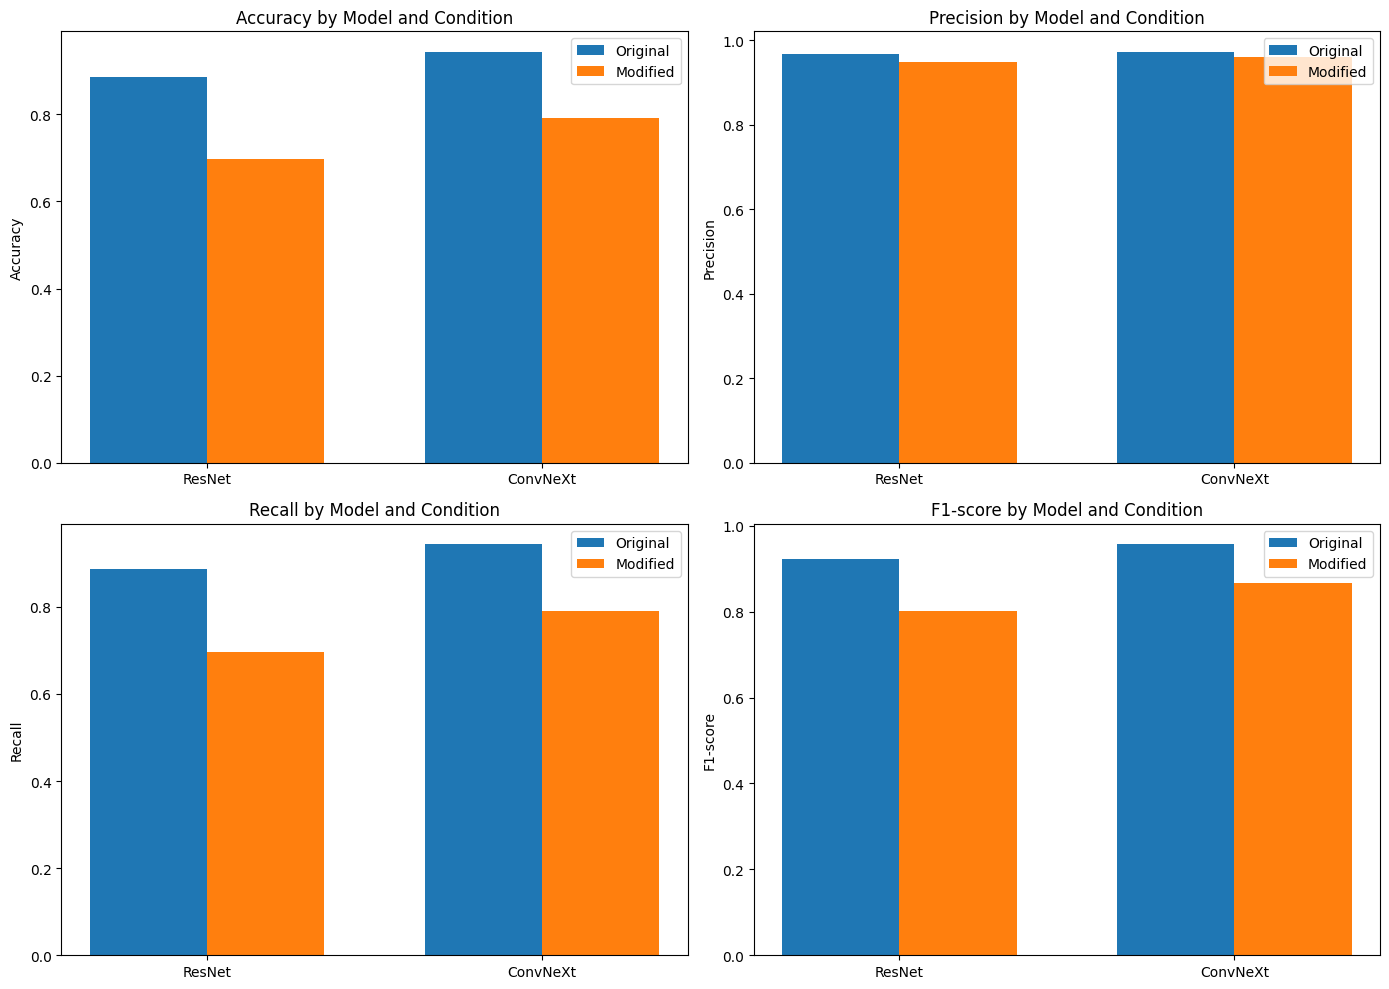
\includegraphics[width=.9\textwidth]{img/overall_metrics}
	\caption{Metryki dla danych oryginalnych zestawionych z danymi o zmodyfikowanych tłach}  
    \label{rys:overall_metrics}
\end{figure}


W badaniach obliczono również średnie wartości confidence scores dla dwóch modeli: ResNet oraz ConvNeXt. Wartości te obejmują ogólną średnią 
confidence score, a także średnie confidence scores dla poprawnych i niepoprawnych klasyfikacji. Dla modelu ResNet na oryginalnych obrazach 
średnia confidence score wyniosła 85.188854, ze średnią wartością 89.137424 dla poprawnych klasyfikacji i 54.348263 dla niepoprawnych. Po 
modyfikacji tła, średnia confidence score spadła do 71.694490, ze średnią wartością 83.929904 dla poprawnych klasyfikacji i 43.546579 dla 
niepoprawnych.

W przypadku modelu ConvNeXt na oryginalnych obrazach średnia confidence score wyniosła 68.527975, ze średnią wartością 70.036361 dla poprawnych 
klasyfikacji i 43.433439 dla niepoprawnych. Po modyfikacji tła, średnia confidence score spadła do 57.543545, ze średnią wartością 63.189640 dla 
poprawnych klasyfikacji i 36.191272 dla niepoprawnych.

Wyniki te wskazują na znaczący spadek średnich confidence scores dla obu modeli po modyfikacji tła. Średnie confidence scores dla poprawnych 
klasyfikacji są wyższe niż dla niepoprawnych w obu przypadkach, co sugeruje, że modele są bardziej pewne swoich poprawnych klasyfikacji. Jednak 
modyfikacja tła powoduje ogólny spadek pewności modeli, co może być wynikiem zmniejszenia jasności sygnałów związanych z obiektami do 
rozpoznania.

Analiza wartości confidence scores dla ConvNeXt wskazuje na większy spadek w porównaniu do ResNet. Model ConvNeXt na oryginalnych obrazach ma 
niższą ogólną średnią confidence score (68.527975) w porównaniu do ResNet (85.188854). Jednakże, spadek ten jest bardziej wyraźny po modyfikacji 
tła, gdzie średnia confidence score dla ConvNeXt wynosi 57.543545, podczas gdy dla ResNet jest to 71.694490.

Podsumowując, modyfikacja tła ma wyraźny wpływ na zmniejszenie pewności klasyfikacji obrazów przez modele ResNet i ConvNeXt. Chociaż oba modele 
wykazują wysoką pewność przy poprawnych klasyfikacjach, modyfikacja tła powoduje ogólny spadek tych wartości, z bardziej zauważalnym spadkiem w 
przypadku modelu ConvNeXt. Wyniki te podkreślają znaczenie zrozumienia i zarządzania wpływem tła na wydajność modeli klasyfikacyjnych w 
praktycznych zastosowaniach.

\begin{table}
	\centering
	\begin{tabular}{|c|c|c|c|c|c|}
		\hline
		\textbf{Model} & \textbf{Type} & \textbf{Average} & 
		\textbf{Average correct} & \textbf{Average incorrect} \\
		\hline
		ResNet & Original & 85.188854 & 89.137424 & 54.348263 \\
		\hline
		ResNet & Modified & 71.694490 & 83.929904 & 43.546579  \\
		\hline
		ConvNeXt & Original & 68.527975 & 70.036361 & 43.433439 \\
		\hline
		ConvNeXt & Modified & 57.543545 & 63.189640 & 36.191272 \\
		\hline
	\end{tabular}
	\caption{Confidence scores dla modeli ResNet i ConvNeXt}
	\label{tab:model_confidence}
\end{table}

\begin{figure}
	\centering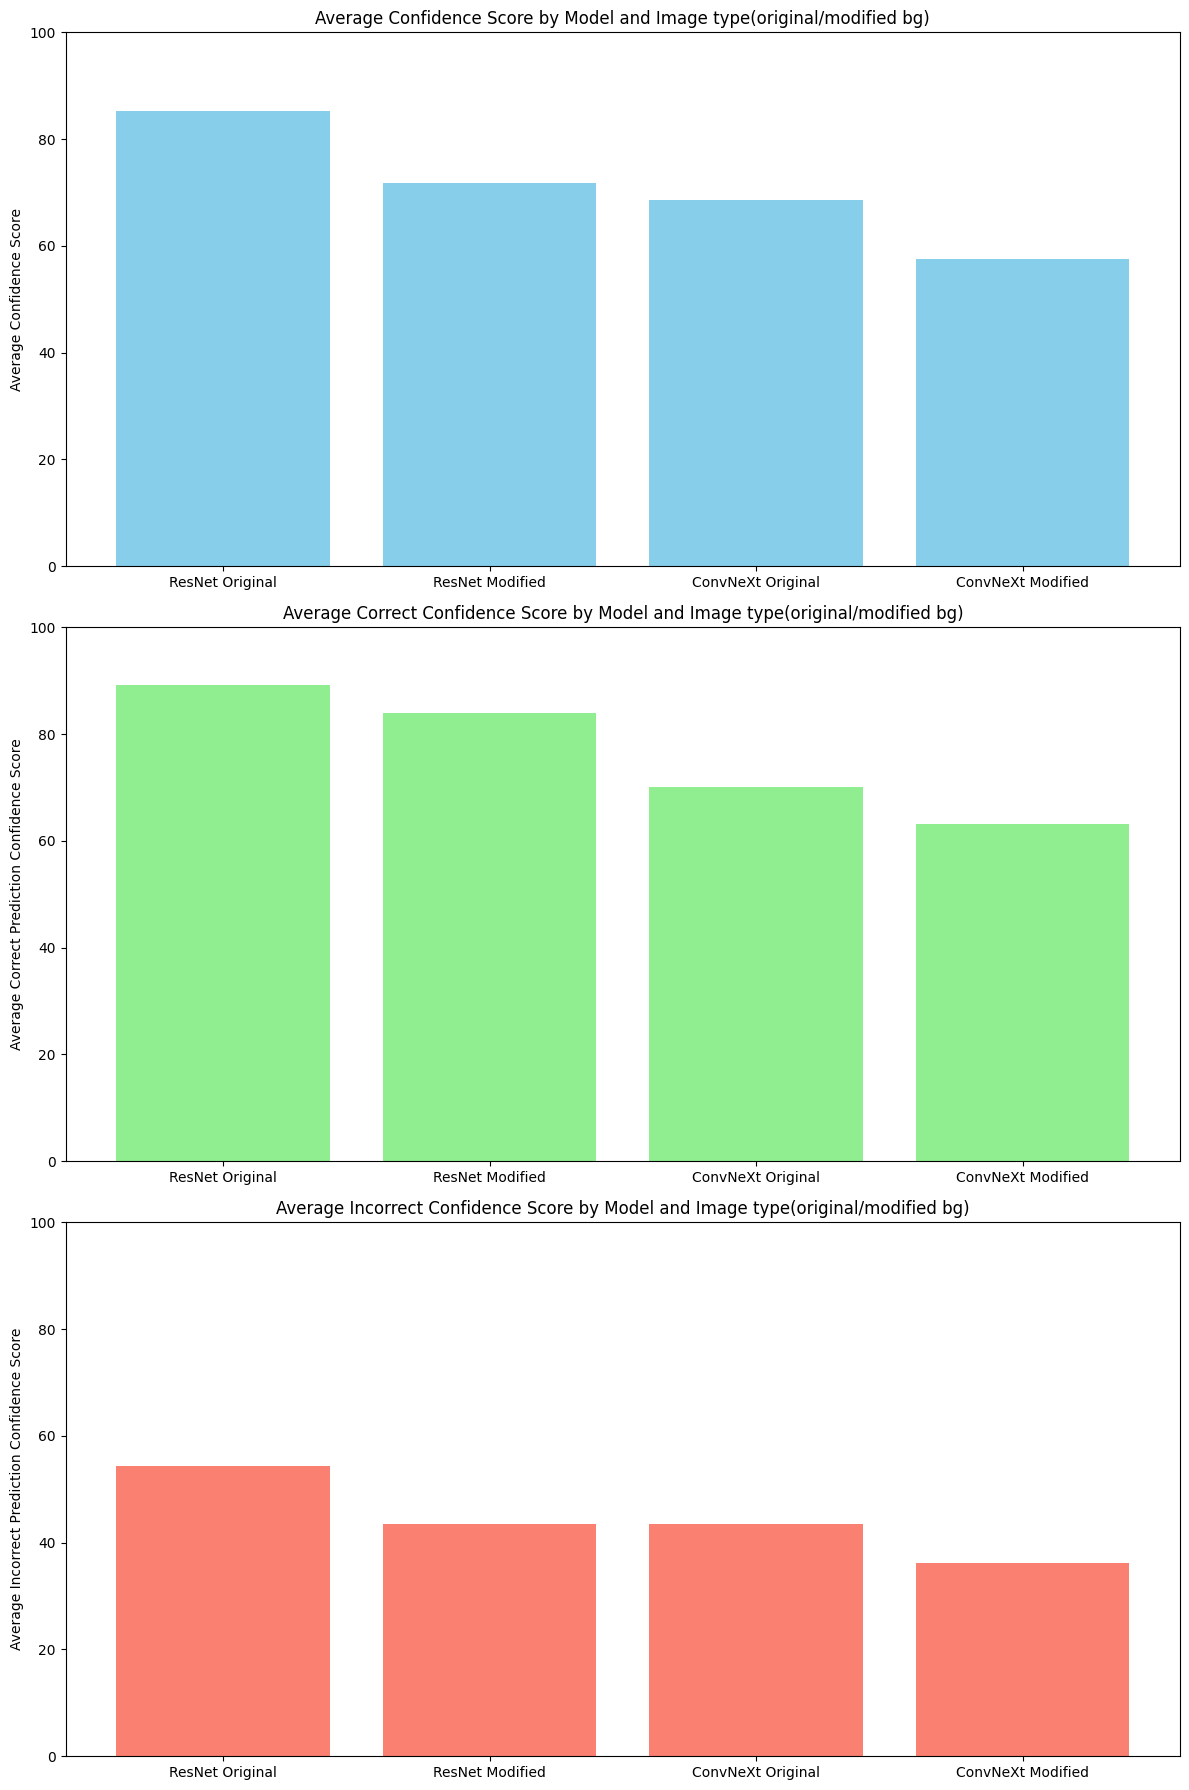
\includegraphics[width=.9\textwidth]{img/confidence_avg}
	\caption{Średnie wartości dla confidence scores}  
    \label{rys:confidence_avg}
\end{figure}
\newpage
Na podstawie dystrybucji confidence scores dla modeli ResNet i ConvNeXt można wyciągnąć kilka istotnych wniosków. Model ResNet wykazuje wysoką 
pewność dla poprawnych klasyfikacji, z koncentracją confidence scores w przedziale od 80 do 100, co wskazuje na jego stabilność w 
identyfikowaniu prawidłowych przypadków. W przypadku błędnych klasyfikacji confidence scores są bardziej równomiernie rozłożone, co oznacza, 
że model jest mniej pewny, gdy się myli. Z kolei model ConvNeXt ma szerszy rozkład confidence scores, z wyraźnym pikiem dla poprawnych 
klasyfikacji w przedziale 70-80 i dla błędnych w przedziale 30-40. Sugeruje to, że ConvNeXt jest mniej pewny swoich poprawnych decyzji w 
porównaniu do ResNet i bardziej skłonny do popełniania błędów z dużą pewnością. Te różnice w rozkładzie pewności klasyfikacji wskazują, że 
ResNet jest bardziej stabilny, podczas gdy ConvNeXt wykazuje większą różnorodność w pewności decyzji, co może wpływać na jego wydajność w 
obliczu modyfikacji tła.

\begin{figure}
	\centering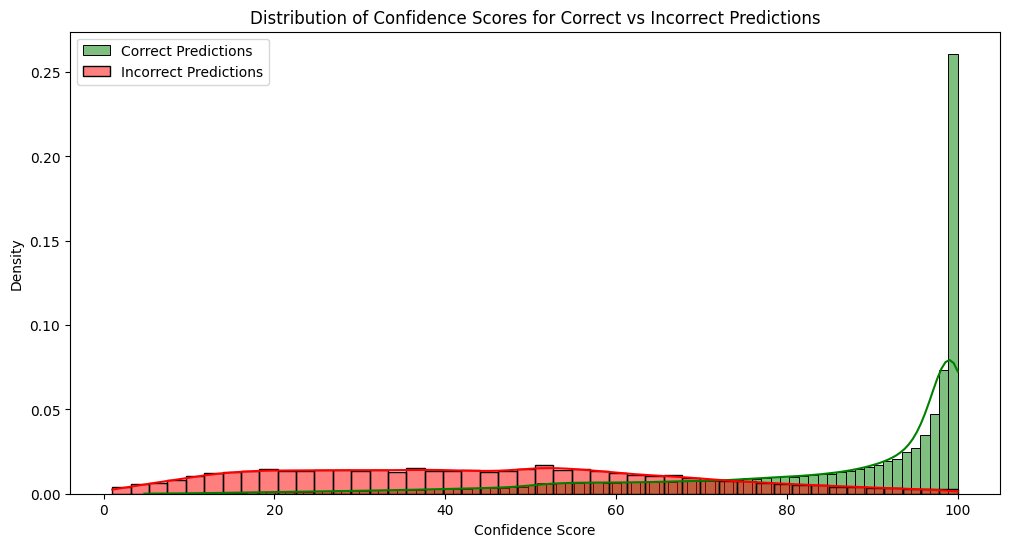
\includegraphics[width=.9\textwidth]{img/resnet_conf_distro}
	\caption{Dystrybucja confidence score dla ResNet}
	\label{rys:res_c_distro}
\end{figure}

\begin{figure}
	\centering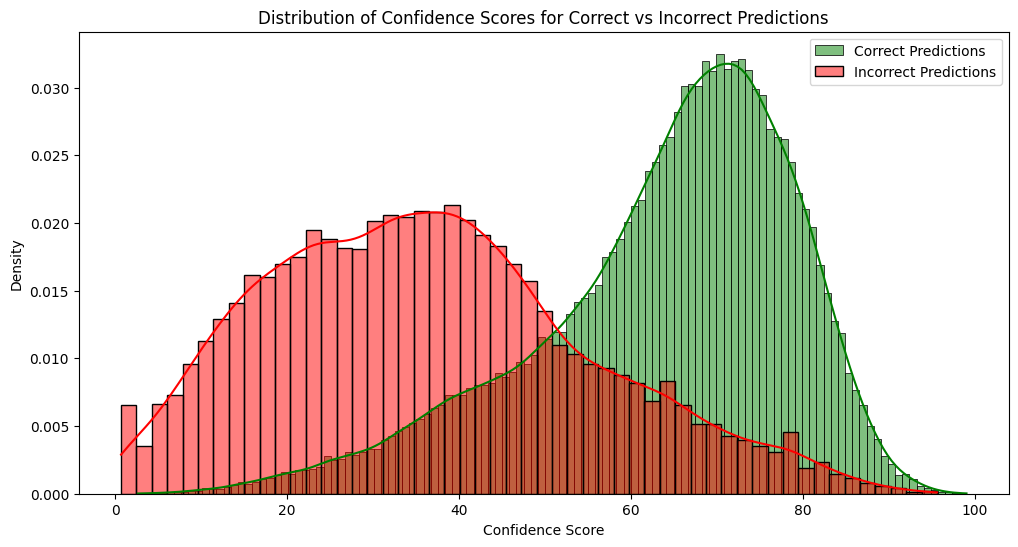
\includegraphics[width=.9\textwidth]{img/convnext_conf_distro}
	\caption{Dystrybucja confidence score dla ConvNext}
	\label{rys:conv_c_distro}
\end{figure}
\newpage

\section*{Wyniki względem kategorii wielkości obiektu}
Analiza wpływu wielkości obiektu na skuteczność klasyfikacji obrazów jest istotnym elementem badań, ponieważ różne rozmiary obiektów mogą 
znacząco wpływać na wydajność modeli głębokiego uczenia. Obiekty o różnych wielkościach mogą być różnie traktowane przez modele klasyfikacyjne 
ze względu na zmienność cech charakterystycznych oraz tła. Dlatego też, zrozumienie, jak zmienia się skuteczność modeli ResNet i ConvNeXt w 
zależności od wielkości obiektu, jest kluczowe dla optymalizacji i poprawy tych modeli w rzeczywistych zastosowaniach.



\begin{table}
	\centering
	\begin{tabular}{|c|c|c|c|c|c|}
		\hline
		\textbf{Object Size} & \textbf{Dataset Type} & \textbf{Accuracy} & \textbf{Precision} & \textbf{Recall} & \textbf{F1-score} \\
		\hline
		Large & Original & 0.877353 & 0.972679 & 0.877353 & 0.920111 \\
		\hline
		Large & Modified & 0.782460 & 0.960542 & 0.782460 & 0.861260 \\
		\hline
		Medium & Original & 0.897879 & 0.963620 & 0.897879 & 0.927600 \\
		\hline
		Medium & Modified & 0.757796 & 0.943584 & 0.757796 & 0.838421 \\
		\hline
		Small & Original & 0.884545 & 0.963823 & 0.884545 & 0.918217 \\
		\hline
		Small & Modified & 0.548209 & 0.936858 & 0.548209 & 0.683307 \\
		\hline
	\end{tabular}
	\caption{Metryki porównawcze modelu ResNet w zależności od wielkości obiektu}
	\label{tab:resnet_object_size_metrics}
\end{table}

Dla modelu ResNet wyniki pokazują, że dla dużych obiektów na oryginalnych obrazach uzyskano Accuracy na poziomie 0.877353, Precision 0.972679, 
Recall 0.877353 i F1-score 0.920111. Po modyfikacji tła wartości te spadły odpowiednio do 0.782460, 0.960542, 0.782460 i 0.861260. Dla obiektów 
średniej wielkości na oryginalnych obrazach uzyskano Accuracy 0.897879, Precision 0.963620, Recall 0.897879 i F1-score 0.927600, a po modyfikacji 
tła wartości te spadły do 0.757796, 0.943584, 0.757796 i 0.838421. Dla małych obiektów na oryginalnych obrazach uzyskano Accuracy 0.884545, 
Precision 0.963823, Recall 0.884545 i F1-score 0.918217, natomiast po modyfikacji tła wartości te drastycznie spadły do 0.548209, 0.936858, 
0.548209 i 0.683307.

Dla modelu ConvNeXt wyniki pokazują, że dla dużych obiektów na oryginalnych obrazach uzyskano Accuracy na poziomie 0.932353, Precision 0.974247, 
Recall 0.932353 i F1-score 0.952076. Po modyfikacji tła wartości te spadły odpowiednio do 0.838610, 0.970077, 0.838610 i 0.897830. Dla obiektów 
średniej wielkości na oryginalnych obrazach uzyskano Accuracy 0.943333, Precision 0.970287, Recall 0.943333 i F1-score 0.955907, a po modyfikacji 
tła wartości te spadły do 0.834545, 0.959503, 0.834545 i 0.888990. Dla małych obiektów na oryginalnych obrazach uzyskano Accuracy 0.954545, 
Precision 0.972766, Recall 0.954545 i F1-score 0.961567, natomiast po modyfikacji tła wartości te spadły do 0.698017, 0.951014, 0.698017 i 0.799677.

\begin{table}
	\centering
	\begin{tabular}{|c|c|c|c|c|c|}
		\hline
		\textbf{Object Size} & \textbf{Dataset Type} & \textbf{Accuracy} & \textbf{Precision} & \textbf{Recall} & \textbf{F1-score} \\
		\hline
		Large & Original & 0.932353 & 0.974247 & 0.932353 & 0.952076 \\
		\hline
		Large & Modified & 0.838610 & 0.970077 & 0.838610 & 0.897830 \\
		\hline
		Medium & Original & 0.943333 & 0.970287 & 0.943333 & 0.955907 \\
		\hline
		Medium & Modified & 0.834545 & 0.959503 & 0.834545 & 0.888990 \\
		\hline
		Small & Original & 0.954545 & 0.972766 & 0.954545 & 0.961567 \\
		\hline
		Small & Modified & 0.698017 & 0.951014 & 0.698017 & 0.799677 \\
		\hline
	\end{tabular}
	\caption{Metryki porównawcze modelu ConvNeXt w zależności od wielkości obiektu}
	\label{tab:convnext_object_size_metrics}
\end{table}

Analiza wyników pokazuje, że modyfikacja tła wpływa na skuteczność klasyfikacji obrazów dla obu modeli, ale wpływ ten jest zróżnicowany w 
zależności od wielkości obiektu. W przypadku małych obiektów, procentowo jest więcej tła niż w przypadku dużych czy średnich obiektów, co może 
prowadzić do większych spadków w Accuracy i innych metrykach. Model ResNet wykazuje znaczący spadek skuteczności dla małych obiektów po 
modyfikacji tła, co sugeruje, że większa ilość tła może wprowadzać większe zakłócenia w procesie klasyfikacji. To samo zjawisko obserwowane 
jest w przypadku modelu ConvNeXt, choć ten model wykazuje lepszą odporność na zmiany tła niż ResNet, zwłaszcza dla małych obiektów.

Wyniki te podkreślają znaczenie rozważania wielkości obiektów przy projektowaniu i ocenie modeli klasyfikacyjnych, szczególnie w kontekście 
modyfikacji tła. Modele mogą wymagać dodatkowego dostrajania lub augmentacji danych, aby poprawić ich odporność na zmiany tła, co jest 
szczególnie istotne dla zastosowań, gdzie obiekty mogą występować w różnych skalach i warunkach środowiskowych. Zrozumienie, że większy udział 
tła przy małych obiektach może prowadzić do większych zakłóceń, jest kluczowe dla opracowywania bardziej efektywnych algorytmów klasyfikacyjnych, 
które mogą niezawodnie działać w zmiennych warunkach.

\begin{table}
	\centering
	\begin{tabular}{|c|c|c|c|}
		\hline
		\textbf{Object Size} & \textbf{Average Score} & \textbf{Correct Score} & \textbf{Incorrect Score} \\
		\hline
		Large & 76.437807 & 85.211125 & 43.360151 \\
		\hline
		Medium & 76.371553 & 85.131233 & 47.133278 \\
		\hline
		Small & 65.538042 & 82.538231 & 42.420987 \\
		\hline
	\end{tabular}
	\caption{Confidence scores dla modelu ResNet w zależności od wielkości obiektu oraz poprawności predykcji}
	\label{tab:resnet_confidence_scores}
\end{table}

\begin{table}
	\centering
	\begin{tabular}{|c|c|c|c|}
		\hline
		\textbf{Object Size} & \textbf{Average Score} & \textbf{Correct Score} & \textbf{Incorrect Score} \\
		\hline
		Large & 63.942224 & 69.166578 & 35.149080 \\
		\hline
		Medium & 60.220167 & 64.178825 & 38.865913 \\
		\hline
		Small & 51.048190 & 57.051329 & 35.657851 \\
		\hline
	\end{tabular}
	\caption{Confidence scores dla modelu ConvNeXt w zależności od wielkości obiektu oraz poprawności predykcji}
	\label{tab:convnext_confidence_scores}
\end{table}

Analiza confidence scores dla modeli ResNet i ConvNeXt w zależności od wielkości obiektu dostarcza cennych informacji o zachowaniu tych modeli. 
Dla modelu ResNet, średnie confidence scores wynoszą 76.437807 dla dużych obiektów, 76.371553 dla obiektów średniej wielkości i 65.538042 dla 
małych obiektów. Dla poprawnych klasyfikacji confidence scores są odpowiednio wyższe, wynosząc 85.211125, 85.131233 i 82.538231. Dla niepoprawnych 
klasyfikacji wartości te są znacznie niższe: 43.360151, 47.133278 i 42.420987.

W przypadku modelu ConvNeXt, średnie confidence scores są niższe i wynoszą 63.942224 dla dużych obiektów, 60.220167 dla obiektów średniej 
wielkości i 51.048190 dla małych obiektów. Confidence scores dla poprawnych klasyfikacji wynoszą 69.166578, 64.178825 i 57.051329, a dla 
niepoprawnych klasyfikacji są to 35.149080, 38.865913 i 35.657851.

yniki te wskazują, że confidence scores dla poprawnych klasyfikacji są wyższe niż dla niepoprawnych w obu modelach, co jest oczekiwane, 
ponieważ modele mają większą pewność przy poprawnych decyzjach. Jednakże, spadki confidence scores dla małych obiektów są bardziej wyraźne, 
co może wynikać z większego udziału tła w tych obrazach, co prowadzi do większych zakłóceń i trudności w klasyfikacji.

Porównując oba modele, ResNet wykazuje wyższe średnie confidence scores zarówno dla poprawnych, jak i niepoprawnych klasyfikacji w porównaniu 
do ConvNeXt. To sugeruje, że ResNet jest bardziej pewny swoich decyzji, niezależnie od wielkości obiektu.

\section*{Wyniki względem typu modyfikacji tła}

W tej sekcji przeanalizowano wpływ różnych typów modyfikacji tła na skuteczność klasyfikacji obrazów oraz wartości confidence scores dla dwóch 
modeli głębokiego uczenia: ResNet i ConvNeXt. Analiza obejmuje metryki klasyfikacji takie jak accuracy, precision, recall i F1-score oraz 
średnie wartości confidence scores zarówno dla poprawnych, jak i niepoprawnych klasyfikacji. Taka analiza jest kluczowa dla zrozumienia, jak 
różne scenariusze modyfikacji tła wpływają na pewność i skuteczność modeli klasyfikacyjnych.

\begin{table}
	\centering
	\begin{tabular}{|c|c|c|c|c|}
		\hline
		\textbf{Modification Type} & \textbf{Accuracy} & \textbf{Precision} & \textbf{Recall} & \textbf{F1-score} \\
		\hline
		Desert & 0.7582 & 0.956658 & 0.7582 & 0.844717 \\
		\hline
		Low & 0.7835 & 0.957333 & 0.7835 & 0.859445 \\
		\hline
		City & 0.7620 & 0.955729 & 0.7620 & 0.845955 \\
		\hline
		Sky & 0.7577 & 0.951998 & 0.7577 & 0.840614 \\
		\hline
		Jungle & 0.7736 & 0.952716 & 0.7736 & 0.846911 \\
		\hline
		No & 0.1935 & 0.857598 & 0.1935 & 0.260654 \\
		\hline
		High & 0.7757 & 0.952540 & 0.7757 & 0.852606 \\
		\hline
		Water & 0.7198 & 0.950886 & 0.7198 & 0.812003 \\
		\hline
		Snow & 0.7462 & 0.961568 & 0.7462 & 0.833842 \\
		\hline
		Indoor & 0.6990 & 0.950477 & 0.6990 & 0.801644 \\
		\hline
		Mountain & 0.6980 & 0.959372 & 0.6980 & 0.800749 \\
		\hline
	\end{tabular}
	\caption{Metryki według typu modyfikacji dla ResNet}
	\label{tab:resnet_metrics_modification}
\end{table}

\begin{table}
	\centering
	\begin{tabular}{|c|c|c|c|}
		\hline
		\textbf{Modification Type} & \textbf{Average Score} & \textbf{Correct Score} & \textbf{Incorrect Score} \\
		\hline
		Desert & 75.954396 & 84.304869 & 49.770241 \\
		\hline
		Low & 77.879677 & 86.411184 & 47.004688 \\
		\hline
		City & 73.458863 & 84.253234 & 38.898736 \\
		\hline
		Sky & 76.063737 & 84.893389 & 48.452397 \\
		\hline
		Jungle & 77.082096 & 85.830222 & 47.190088 \\
		\hline
		No & 41.084428 & 67.091235 & 34.844729 \\
		\hline
		High & 77.275950 & 86.369482 & 45.827655 \\
		\hline
		Water & 70.044268 & 80.529769 & 43.108282 \\
		\hline
		Snow & 76.379893 & 85.181503 & 50.502187 \\
		\hline
		Indoor & 72.859840 & 83.005442 & 49.299121 \\
		\hline
		Mountain & 70.556246 & 82.283334 & 43.451917 \\
		\hline
	\end{tabular}
	\caption{Confidence Scores według typu modyfikacji dla ResNet}
	\label{tab:resnet_confidence_modification}
\end{table}

\begin{table}
	\centering
	\begin{tabular}{|c|c|c|c|c|}
		\hline
		\textbf{Modification Type} & \textbf{Accuracy} & \textbf{Precision} & \textbf{Recall} & \textbf{F1-score} \\
		\hline
		Desert & 0.8234 & 0.965246 & 0.8234 & 0.885689 \\
		\hline
		Low & 0.8897 & 0.965665 & 0.8897 & 0.925404 \\
		\hline
		City & 0.8392 & 0.967133 & 0.8392 & 0.894941 \\
		\hline
		Sky & 0.8259 & 0.958754 & 0.8259 & 0.886533 \\
		\hline
		Jungle & 0.8621 & 0.963912 & 0.8621 & 0.909624 \\
		\hline
		No & 0.2572 & 0.921080 & 0.2572 & 0.343413 \\
		\hline
		High & 0.8707 & 0.964345 & 0.8707 & 0.913518 \\
		\hline
		Water & 0.8593 & 0.960770 & 0.8593 & 0.906849 \\
		\hline
		Snow & 0.8567 & 0.966667 & 0.8567 & 0.902537 \\
		\hline
		Indoor & 0.7797 & 0.965780 & 0.7797 & 0.859119 \\
		\hline
		Mountain & 0.8357 & 0.964700 & 0.8357 & 0.891118 \\
		\hline
	\end{tabular}
	\caption{Metryki według typu modyfikacji dla ConvNeXt}
	\label{tab:convnext_metrics_modification}
\end{table}

\begin{table}
	\centering
	\begin{tabular}{|c|c|c|c|}
		\hline
		\textbf{Modification Type} & \textbf{Average Score} & \textbf{Correct Score} & \textbf{Incorrect Score} \\
		\hline
		Desert & 61.750625 & 65.260020 & 45.388021 \\
		\hline
		Low & 57.798021 & 61.428446 & 28.514347 \\
		\hline
		City & 58.404538 & 62.933008 & 34.770883 \\
		\hline
		Sky & 56.927464 & 60.928925 & 37.945228 \\
		\hline
		Jungle & 60.313014 & 63.350853 & 41.321559 \\
		\hline
		No & 38.674228 & 56.533386 & 32.490362 \\
		\hline
		High & 57.146265 & 61.220278 & 29.712060 \\
		\hline
		Water & 57.189347 & 60.885762 & 34.614159 \\
		\hline
		Snow & 61.818994 & 65.527449 & 39.648495 \\
		\hline
		Indoor & 61.650110 & 66.519692 & 44.415372 \\
		\hline
		Mountain & 61.306386 & 66.316218 & 35.824236 \\
		\hline
	\end{tabular}
	\caption{Confidence według typu modyfikacji dla ConvNeXt}
	\label{tab:convnext_confidence_modification}
\end{table}

Analiza wyników pokazuje, że typ modyfikacji tła ma znaczący wpływ na skuteczność klasyfikacji obrazów oraz wartości confidence scores dla obu 
modeli. Modele osiągały najwyższą skuteczność i pewność klasyfikacji w scenariuszach, gdzie tło było bardziej uporządkowane lub zawierało mniej 
zakłócających elementów (np. "high", "low", "jungle"). Największe spadki skuteczności i pewności klasyfikacji obserwowano w scenariuszu "no", 
gdzie tło było całkowicie usunięte, co sugeruje, że brak tła może utrudniać modelom identyfikację istotnych cech obiektów.

Wyniki te podkreślają znaczenie uwzględniania różnych typów tła podczas trenowania i oceny modeli klasyfikacyjnych. Zrozumienie, jak różne 
modyfikacje tła wpływają na skuteczność i pewność klasyfikacji, może prowadzić do opracowania bardziej odpornych modeli, które lepiej radzą 
sobie w zróżnicowanych warunkach. Dalsze badania mogą skoncentrować się na metodach augmentacji danych, które mogą poprawić wydajność modeli w 
scenariuszach z różnorodnymi tłami.
\begin{figure}
	\centering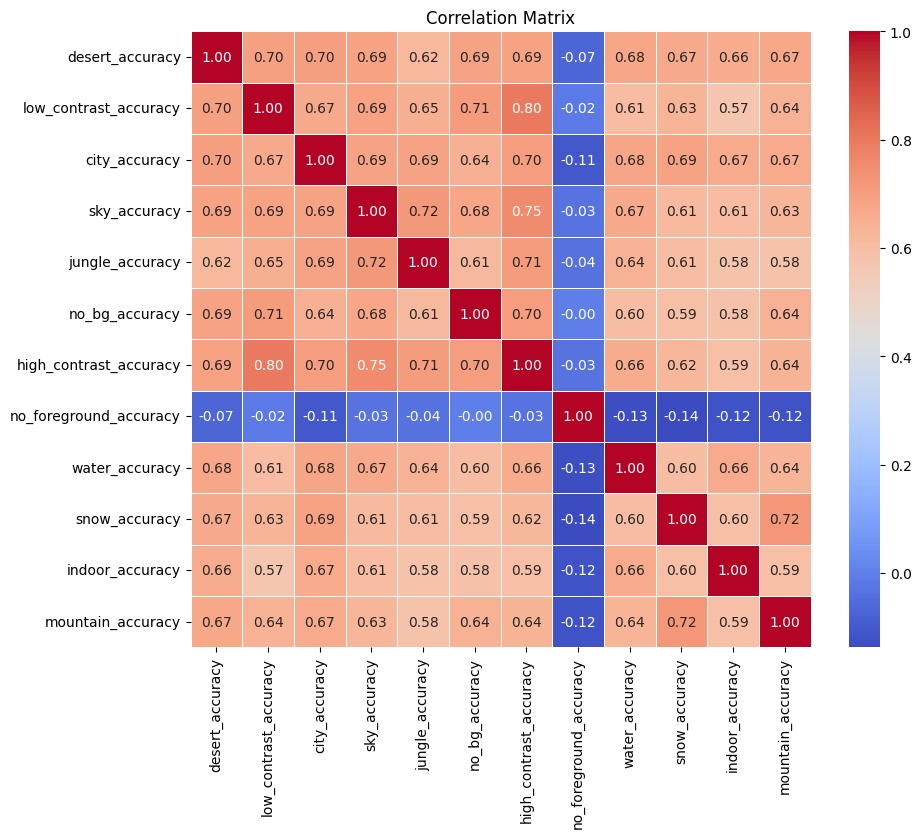
\includegraphics[width=.9\textwidth]{img/korelacja_resnet_typ}
	\caption{Tabela korelacji dla ResNet dla typów modyfikacji}  
    \label{rys:corelation_resnet_type}
\end{figure}

Macierz korelacji dla modelu ResNet pokazuje, jak różne typy modyfikacji tła wpływają 
na wzajemne relacje między wskaźnikami skuteczności (accuracy). Typy modyfikacji 
takie jak "desert", "low", "city", "sky", "high" i "water" wykazują wysoką dodatnią 
korelację między sobą (od 0.67 do 0.80). Oznacza to, że jeżeli model osiąga wysoką 
skuteczność w jednym z tych scenariuszy, prawdopodobnie osiągnie też wysoką 
skuteczność w innych złożonych scenariuszach tła. Z kolei scenariusz "no" 
(bez obiektu, tylko tło) wykazuje niską lub ujemną korelację z innymi typami 
modyfikacji, z korelacjami wahającymi się od -0.13 do 0.12. To wskazuje, że obecność 
tylko tła, bez obiektu, ma zupełnie odmienny wpływ na skuteczność modelu w porównaniu 
do innych scenariuszy tła. Wysoka korelacja (0.80) między "low" a "high" sugeruje, 
że model działa podobnie w obu tych typach modyfikacji, które mimo różnic w 
strukturze tła mają podobny wpływ na jego skuteczność.

Macierz korelacji dla modelu ConvNeXt również pokazuje, jak różne typy modyfikacji 
tła wpływają na wzajemne relacje między wskaźnikami skuteczności (accuracy). 
Typy modyfikacji takie jak "desert", "low", "city", "sky", "jungle", "high", "water", 
"snow" i "mountain" wykazują wysoką dodatnią korelację (od 0.64 do 0.81). 
Sugeruje to, że model ConvNeXt ma zdolność adaptacji do różnych złożonych środowisk, 
osiągając zbliżone wyniki w różnych warunkach tła. Z kolei scenariusz "no" 
(bez obiektu, tylko tło) wykazuje ujemną korelację z innymi typami modyfikacji, 
szczególnie z "desert", "city" i "mountain" (od -0.17 do -0.15), co oznacza, że 
obecność tylko tła znacząco obniża skuteczność modelu ConvNeXt. Wysoka korelacja 
(0.81) między "low" a "high", podobnie jak w modelu ResNet, sugeruje, że ConvNeXt 
działa dobrze w scenariuszach z minimalnymi zakłóceniami w tle. Jednak model ten 
wykazuje również wysoką korelację między "city" a "mountain" (0.80), co wskazuje na 
jego zdolność do adaptacji w bardziej różnorodnych i strukturalnych warunkach tła.

\begin{figure}
	\centering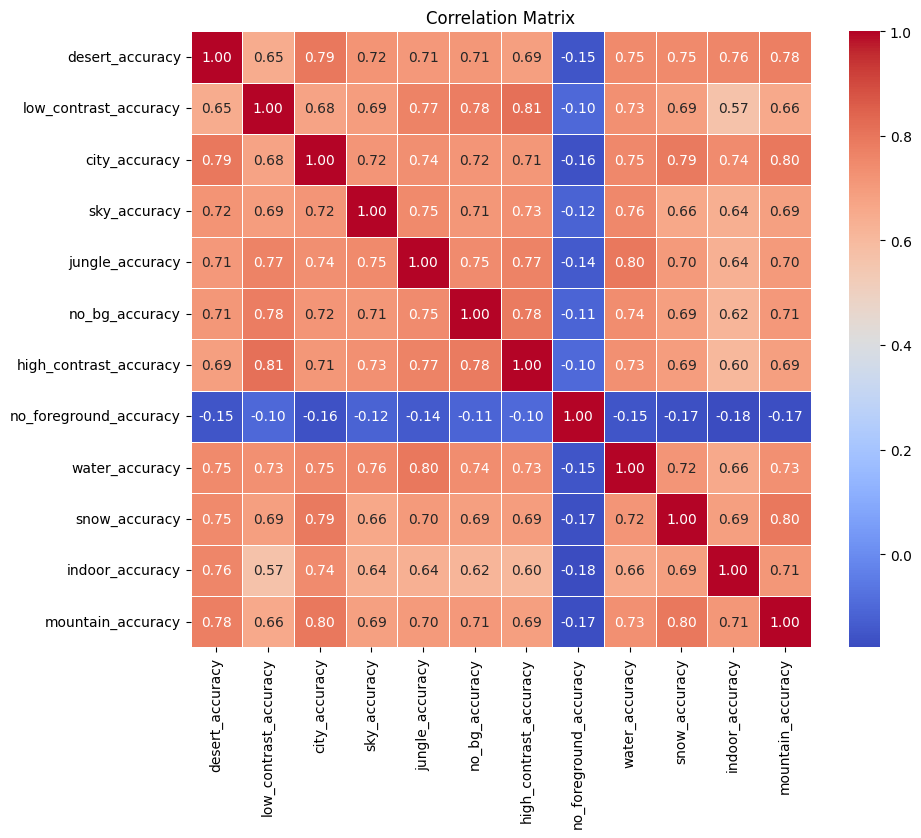
\includegraphics[width=.9\textwidth]{img/korelacja_convnext_typ}
	\caption{Tabela korelacji dla ConvNeXt dla typów modyfikacji}  
    \label{rys:corelation_convnext_type}
\end{figure}

\section*{Wyniki względem klas}

\begin{table}
	\centering
	\begin{tabular}{|c|c|c|c|}
		\hline
		\textbf{Modification Type} & \textbf{Accuracy} & \textbf{Avg Confidence} & \textbf{Most Mistaken} \\
		\hline
		Original & 0.781 & 80.888742 & Bighorn, bighorn sheep \\
		\hline
		Desert & 0.662 & 73.618091 & Bighorn, bighorn sheep \\
		\hline
		Low & 0.637 & 72.533478 & Bighorn, bighorn sheep \\
		\hline
		City & 0.691 & 71.055787 & Bighorn, bighorn sheep \\
		\hline
		Sky & 0.752 & 74.196770 & Bighorn, bighorn sheep \\
		\hline
		Jungle & 0.825 & 76.201070 & Bighorn, bighorn sheep \\
		\hline
		No & 0.136 & 38.340821 & American black bear, black bear \\
		\hline
		High & 0.735 & 73.587178 & Bighorn, bighorn sheep \\
		\hline
		Water & 0.780 & 72.729140 & Bighorn, bighorn sheep \\
		\hline
		Snow & 0.601 & 76.547279 & Bighorn, bighorn sheep \\
		\hline
		Indoor & 0.683 & 71.596914 & Bighorn, bighorn sheep \\
		\hline
		Mountain & 0.613 & 74.327448 & Bighorn, bighorn sheep \\
		\hline
	\end{tabular}
	\caption{Metrics and Confidence Scores for Class 348 (ram, tup) - ResNet}
	\label{tab:metrics_confidence_class_348_resnet}
\end{table}

\begin{table}
	\centering
	\begin{tabular}{|c|c|c|c|}
		\hline
		\textbf{Modification Type} & \textbf{Accuracy} & \textbf{Avg Confidence} & \textbf{Most Mistaken} \\
		\hline
		Original & 0.801 & 64.573134 & Bighorn, bighorn sheep \\
		\hline
		Desert & 0.589 & 59.293923 & Bighorn, bighorn sheep \\
		\hline
		Low & 0.752 & 57.574512 & Bighorn, bighorn sheep \\
		\hline
		City & 0.604 & 57.563126 & Bighorn, bighorn sheep \\
		\hline
		Sky & 0.717 & 57.364283 & Bighorn, bighorn sheep \\
		\hline
		Jungle & 0.747 & 60.548807 & Bighorn, bighorn sheep \\
		\hline
		No & 0.274 & 36.891416 & American black bear, black bear \\
		\hline
		High & 0.706 & 56.227286 & Bighorn, bighorn sheep \\
		\hline
		Water & 0.745 & 57.906020 & Bighorn, bighorn sheep \\
		\hline
		Snow & 0.580 & 59.995922 & Bighorn, bighorn sheep \\
		\hline
		Indoor & 0.556 & 59.476196 & Bighorn, bighorn sheep \\
		\hline
		Mountain & 0.588 & 61.288639 & Bighorn, bighorn sheep \\
		\hline
	\end{tabular}
	\caption{Metrics and Confidence Scores for Class 348 (ram, tup) - ConvNeXt}
	\label{tab:metrics_confidence_class_348_convnext}
\end{table}

\begin{table}
	\centering
	\begin{tabular}{|c|c|c|c|}
		\hline
		\textbf{Modification Type} & \textbf{Accuracy} & \textbf{Avg Confidence} & \textbf{Most Mistaken For} \\
		\hline
		Original & 0.746 & 69.254460 & EntleBucher \\
		\hline
		Desert & 0.751 & 71.670600 & EntleBucher \\
		\hline
		Low & 0.628 & 66.772043 & EntleBucher \\
		\hline
		City & 0.720 & 70.455594 & Appenzeller \\
		\hline
		Sky & 0.693 & 67.656871 & EntleBucher \\
		\hline
		Jungle & 0.680 & 66.612556 & EntleBucher \\
		\hline
		No & 0.009 & 29.458587 & American black bear, black bear \\
		\hline
		High & 0.632 & 65.697515 & Appenzeller \\
		\hline
		Water & 0.679 & 65.613398 & Appenzeller \\
		\hline
		Snow & 0.748 & 71.034704 & EntleBucher \\
		\hline
		Indoor & 0.750 & 71.739733 & EntleBucher \\
		\hline
		Mountain & 0.605 & 63.748537 & EntleBucher \\
		\hline
	\end{tabular}
	\caption{Metrics and Confidence Scores for Class 238 (Greater Swiss Mountain Dog) - ResNet}
	\label{tab:metrics_confidence_class_238_resnet}
\end{table}

\begin{table}
	\centering
	\begin{tabular}{|c|c|c|c|}
		\hline
		\textbf{Modification Type} & \textbf{Accuracy} & \textbf{Avg Confidence} & \textbf{Most Mistaken For} \\
		\hline
		Original & 0.918 & 67.297499 & EntleBucher \\
		\hline
		Desert & 0.812 & 53.915638 & EntleBucher \\
		\hline
		Low & 0.857 & 53.678023 & Appenzeller \\
		\hline
		City & 0.845 & 55.105653 & Appenzeller \\
		\hline
		Sky & 0.784 & 52.714931 & EntleBucher \\
		\hline
		Jungle & 0.853 & 57.766105 & Appenzeller \\
		\hline
		No & 0.036 & 31.021854 & Labrador retriever \\
		\hline
		High & 0.790 & 49.376622 & Appenzeller \\
		\hline
		Water & 0.868 & 55.700216 & Appenzeller \\
		\hline
		Snow & 0.893 & 61.105172 & EntleBucher \\
		\hline
		Indoor & 0.815 & 61.047711 & Bookcase \\
		\hline
		Mountain & 0.850 & 61.289471 & Appenzeller \\
		\hline
	\end{tabular}
	\caption{Metrics and Confidence Scores for Class 238 (Greater Swiss Mountain Dog) - ConvNeXt}
	\label{tab:metrics_confidence_class_238_convnext}
\end{table}

\begin{table}
	\centering
	\begin{tabular}{|c|c|c|c|}
		\hline
		\textbf{Modification Type} & \textbf{Accuracy} & \textbf{Avg Confidence} & \textbf{Most Mistaken For} \\
		\hline
		Original & 0.963 & 95.023629 & Jacamar \\
		\hline
		Desert & 0.677 & 73.851502 & Seashore, coast \\
		\hline
		Low & 0.836 & 83.892216 & Kite \\
		\hline
		City & 0.649 & 63.584482 & Flagpole, flagstaff \\
		\hline
		Sky & 0.789 & 81.238139 & Volcano \\
		\hline
		Jungle & 0.796 & 80.272471 & Greenhouse, nursery \\
		\hline
		No & 0.744 & 69.953177 & Vulture \\
		\hline
		High & 0.782 & 79.808579 & Kite \\
		\hline
		Water & 0.525 & 60.158964 & Albatross, mollymawk \\
		\hline
		Snow & 0.543 & 63.296984 & Snowmobile \\
		\hline
		Indoor & 0.565 & 66.628743 & File, file cabinet \\
		\hline
		Mountain & 0.456 & 54.866228 & Lakeside, lakeshore \\
		\hline
	\end{tabular}
	\caption{Metrics and Confidence Scores for Class 94 (Hummingbird) - ResNet}
	\label{tab:metrics_confidence_class_94_resnet}
\end{table}

\begin{table}
	\centering
	\begin{tabular}{|c|c|c|c|}
		\hline
		\textbf{Modification Type} & \textbf{Accuracy} & \textbf{Avg Confidence} & \textbf{Most Mistaken For} \\
		\hline
		Original & 0.995 & 72.907262 & Jacamar \\
		\hline
		Desert & 0.805 & 63.267602 & Arabian camel, dromedary \\
		\hline
		Low & 0.928 & 57.850450 & Matchstick \\
		\hline
		City & 0.826 & 56.319503 & Traffic light, traffic signal \\
		\hline
		Sky & 0.848 & 57.166515 & Parachute, chute \\
		\hline
		Jungle & 0.859 & 61.211524 & Cliff, drop \\
		\hline
		No & 0.868 & 67.694296 & Jacamar \\
		\hline
		High & 0.911 & 56.167147 & Kite \\
		\hline
		Water & 0.821 & 56.428329 & Albatross, mollymawk \\
		\hline
		Snow & 0.801 & 60.554314 & Lakeside, lakeshore \\
		\hline
		Indoor & 0.718 & 57.200175 & File, file cabinet \\
		\hline
		Mountain & 0.774 & 59.565332 & Valley, vale \\
		\hline
	\end{tabular}
	\caption{Metrics and Confidence Scores for Class 94 (Hummingbird) - ConvNeXt}
	\label{tab:metrics_confidence_class_94_convnext}
\end{table}

\begin{table}
	\centering
	\begin{tabular}{|c|c|c|c|}
		\hline
		\textbf{Modification Type} & \textbf{Accuracy} & \textbf{Avg Confidence} & \textbf{Most Mistaken For} \\
		\hline
		Original & 0.782 & 73.471966 & Tabby, tabby cat \\
		\hline
		Desert & 0.825 & 76.229713 & Tabby, tabby cat \\
		\hline
		Low & 0.821 & 78.051673 & Tabby, tabby cat \\
		\hline
		City & 0.763 & 71.972776 & Tabby, tabby cat \\
		\hline
		Sky & 0.766 & 71.577528 & Tabby, tabby cat \\
		\hline
		Jungle & 0.698 & 70.001732 & Tiger cat \\
		\hline
		No & 0.260 & 33.898078 & Quilt, comforter \\
		\hline
		High & 0.794 & 77.981898 & Tabby, tabby cat \\
		\hline
		Water & 0.846 & 75.972695 & Tabby, tabby cat \\
		\hline
		Snow & 0.647 & 67.339146 & Tiger cat \\
		\hline
		Indoor & 0.743 & 74.809806 & Tabby, tabby cat \\
		\hline
		Mountain & 0.730 & 67.302426 & Tabby, tabby cat \\
		\hline
	\end{tabular}
	\caption{Metrics and Confidence Scores for Class 285 (Egyptian Cat) - ResNet}
	\label{tab:metrics_confidence_class_285_resnet}
\end{table}

\begin{table}
	\centering
	\begin{tabular}{|c|c|c|c|}
		\hline
		\textbf{Modification Type} & \textbf{Accuracy} & \textbf{Avg Confidence} & \textbf{Most Mistaken For} \\
		\hline
		Original & 0.875 & 67.470651 & Tabby, tabby cat \\
		\hline
		Desert & 0.840 & 64.843979 & Tabby, tabby cat \\
		\hline
		Low & 0.842 & 60.234300 & Tabby, tabby cat \\
		\hline
		City & 0.788 & 58.385278 & Tabby, tabby cat \\
		\hline
		Sky & 0.783 & 55.255898 & Tabby, tabby cat \\
		\hline
		Jungle & 0.816 & 59.110254 & Tabby, tabby cat \\
		\hline
		No & 0.301 & 36.188940 & Schipperke \\
		\hline
		High & 0.816 & 60.301645 & Tabby, tabby cat \\
		\hline
		Water & 0.862 & 58.187896 & Tabby, tabby cat \\
		\hline
		Snow & 0.823 & 59.457130 & Tabby, tabby cat \\
		\hline
		Indoor & 0.724 & 62.997077 & Bookcase \\
		\hline
		Mountain & 0.829 & 58.399331 & Tabby, tabby cat \\
		\hline
	\end{tabular}
	\caption{Metrics and Confidence Scores for Class 285 (Egyptian Cat) - ConvNeXt}
	\label{tab:metrics_confidence_class_285_convnext}
\end{table}

\begin{table}
	\centering
	\begin{tabular}{|c|c|c|c|}
		\hline
		\textbf{Modification Type} & \textbf{Accuracy} & \textbf{Avg Confidence} & \textbf{Most Mistaken For} \\
		\hline
		Original & 0.857 & 76.879462 & Ram, tup \\
		\hline
		Desert & 0.644 & 65.576020 & Seashore, coast \\
		\hline
		Low & 0.707 & 62.688885 & Ram, tup \\
		\hline
		City & 0.583 & 57.522109 & Ram, tup \\
		\hline
		Sky & 0.501 & 61.268969 & Ram, tup \\
		\hline
		Jungle & 0.471 & 59.756806 & Ram, tup \\
		\hline
		No & 0.300 & 46.576951 & American black bear, black bear \\
		\hline
		High & 0.583 & 59.381386 & Ram, tup \\
		\hline
		Water & 0.457 & 58.803368 & Ram, tup \\
		\hline
		Snow & 0.783 & 72.009580 & Alp \\
		\hline
		Indoor & 0.467 & 60.394391 & Ram, tup \\
		\hline
		Mountain & 0.725 & 66.198482 & Ram, tup \\
		\hline
	\end{tabular}
	\caption{Metrics and Confidence Scores for Class 349 (Bighorn Sheep) - ResNet}
	\label{tab:metrics_confidence_class_349_resnet}
\end{table}

\begin{table}
	\centering
	\begin{tabular}{|c|c|c|c|}
		\hline
		\textbf{Modification Type} & \textbf{Accuracy} & \textbf{Avg Confidence} & \textbf{Most Mistaken For} \\
		\hline
		Original & 0.908 & 56.144302 & Ram, tup \\
		\hline
		Desert & 0.739 & 53.343471 & Arabian camel, dromedary \\
		\hline
		Low & 0.792 & 43.160569 & Ram, tup \\
		\hline
		City & 0.814 & 48.102590 & Traffic light, traffic signal \\
		\hline
		Sky & 0.660 & 44.070363 & Ram, tup \\
		\hline
		Jungle & 0.709 & 47.144147 & Ram, tup \\
		\hline
		No & 0.369 & 41.866028 & American black bear, black bear \\
		\hline
		High & 0.786 & 42.740627 & Ram, tup \\
		\hline
		Water & 0.714 & 44.812545 & Ram, tup \\
		\hline
		Snow & 0.878 & 55.639899 & Lakeside, lakeshore \\
		\hline
		Indoor & 0.715 & 51.461317 & File, file cabinet \\
		\hline
		Mountain & 0.826 & 53.093244 & Valley, vale \\
		\hline
	\end{tabular}
	\caption{Metrics and Confidence Scores for Class 349 (Bighorn Sheep) - ConvNeXt}
	\label{tab:metrics_confidence_class_349_convnext}
\end{table}

\begin{table}
	\centering
	\begin{tabular}{|c|c|c|c|}
		\hline
		\textbf{Modification Type} & \textbf{Accuracy} & \textbf{Avg Confidence} & \textbf{Most Mistaken For} \\
		\hline
		Original & 0.941 & 88.632230 & Tibetan terrier, chrysanthemum dog \\
		\hline
		Desert & 0.801 & 80.359347 & Seashore, coast \\
		\hline
		Low & 0.785 & 77.904651 & Sealyham terrier, Sealyham \\
		\hline
		City & 0.765 & 74.680369 & Cab, hack \\
		\hline
		Sky & 0.718 & 74.347288 & Volcano \\
		\hline
		Jungle & 0.782 & 75.977385 & Greenhouse, nursery \\
		\hline
		No & 0.071 & 31.629389 & American black bear, black bear \\
		\hline
		High & 0.760 & 75.577558 & Sealyham terrier, Sealyham \\
		\hline
		Water & 0.758 & 76.056336 & Albatross, mollymawk \\
		\hline
		Snow & 0.803 & 80.582623 & Alp \\
		\hline
		Indoor & 0.824 & 84.001364 & File, file cabinet \\
		\hline
		Mountain & 0.715 & 70.130826 & Valley, vale \\
		\hline
	\end{tabular}
	\caption{Metrics and Confidence Scores for Class 229 (Old English Sheepdog) - ResNet}
	\label{tab:metrics_confidence_class_229_resnet}
\end{table}

\begin{table}
	\centering
	\begin{tabular}{|c|c|c|c|}
		\hline
		\textbf{Modification Type} & \textbf{Accuracy} & \textbf{Avg Confidence} & \textbf{Most Mistaken For} \\
		\hline
		Original & 0.987 & 74.735155 & Collie \\
		\hline
		Desert & 0.871 & 66.845438 & Arabian camel, dromedary \\
		\hline
		Low & 0.910 & 60.380093 & Matchstick \\
		\hline
		City & 0.882 & 63.133430 & Traffic light, traffic signal \\
		\hline
		Sky & 0.824 & 56.268607 & Volcano \\
		\hline
		Jungle & 0.890 & 64.798835 & Cliff, drop \\
		\hline
		No & 0.109 & 32.475152 & Newfoundland, Newfoundland dog \\
		\hline
		High & 0.891 & 59.879026 & Matchstick \\
		\hline
		Water & 0.879 & 60.280609 & Grey whale, gray whale \\
		\hline
		Snow & 0.896 & 64.967973 & Lakeside, lakeshore \\
		\hline
		Indoor & 0.867 & 69.414455 & Bookcase \\
		\hline
		Mountain & 0.856 & 62.675450 & Valley, vale \\
		\hline
	\end{tabular}
	\caption{Metrics and Confidence Scores for Class 229 (Old English Sheepdog) - ConvNeXt}
	\label{tab:metrics_confidence_class_229_convnext}
\end{table}

\begin{table}
	\centering
	\begin{tabular}{|c|c|c|c|}
		\hline
		\textbf{Modification Type} & \textbf{Accuracy} & \textbf{Avg Confidence} & \textbf{Most Mistaken For} \\
		\hline
		Original & 0.964 & 93.028729 & Angora, Angora rabbit \\
		\hline
		Desert & 0.848 & 83.349976 & Seashore, coast \\
		\hline
		Low & 0.855 & 83.713232 & Tabby, tabby cat \\
		\hline
		City & 0.877 & 84.163735 & Tabby, tabby cat \\
		\hline
		Sky & 0.821 & 82.203083 & Volcano \\
		\hline
		Jungle & 0.831 & 81.888781 & Greenhouse, nursery \\
		\hline
		No & 0.025 & 23.772934 & Quilt, comforter \\
		\hline
		High & 0.853 & 84.050749 & Tabby, tabby cat \\
		\hline
		Water & 0.821 & 79.093091 & Albatross, mollymawk \\
		\hline
		Snow & 0.829 & 82.849727 & Alp \\
		\hline
		Indoor & 0.879 & 87.654082 & File, file cabinet \\
		\hline
		Mountain & 0.794 & 77.893145 & Valley, vale \\
		\hline
	\end{tabular}
	\caption{Metrics and Confidence Scores for Class 283 (Persian Cat) - ResNet}
	\label{tab:metrics_confidence_class_283_resnet}
\end{table}

\begin{table}
	\centering
	\begin{tabular}{|c|c|c|c|}
		\hline
		\textbf{Modification Type} & \textbf{Accuracy} & \textbf{Avg Confidence} & \textbf{Most Mistaken For} \\
		\hline
		Original & 0.991 & 75.141474 & Feather boa, boa \\
		\hline
		Desert & 0.914 & 70.630613 & Arabian camel, dromedary \\
		\hline
		Low & 0.947 & 66.190509 & Matchstick \\
		\hline
		City & 0.936 & 68.423853 & Traffic light, traffic signal \\
		\hline
		Sky & 0.887 & 63.020165 & Volcano \\
		\hline
		Jungle & 0.925 & 67.672465 & Cliff, drop \\
		\hline
		No & 0.061 & 25.145970 & Schipperke \\
		\hline
		High & 0.942 & 68.444946 & Corkscrew, bottle screw \\
		\hline
		Water & 0.906 & 59.895699 & Grey whale, gray whale \\
		\hline
		Snow & 0.925 & 67.393982 & Lakeside, lakeshore \\
		\hline
		Indoor & 0.907 & 72.101543 & Bookcase \\
		\hline
		Mountain & 0.916 & 67.004423 & Valley, vale \\
		\hline
	\end{tabular}
	\caption{Metrics and Confidence Scores for Class 283 (Persian Cat) - ConvNeXt}
	\label{tab:metrics_confidence_class_283_convnext}
\end{table}

\begin{table}
	\centering
	\begin{tabular}{|c|c|c|c|}
		\hline
		\textbf{Modification Type} & \textbf{Accuracy} & \textbf{Avg Confidence} & \textbf{Most Mistaken For} \\
		\hline
		Original & 0.976 & 95.314826 & House finch, linnet \\
		\hline
		Desert & 0.839 & 81.161059 & Seashore, coast \\
		\hline
		Low & 0.877 & 86.390556 & Brambling, Fringilla montifringilla \\
		\hline
		City & 0.842 & 75.437180 & House finch, linnet \\
		\hline
		Sky & 0.842 & 83.426079 & Volcano \\
		\hline
		Jungle & 0.920 & 90.342285 & Bittern \\
		\hline
		No & 0.362 & 51.447448 & Water ouzel, dipper \\
		\hline
		High & 0.896 & 87.080903 & Kite \\
		\hline
		Water & 0.716 & 61.873004 & Albatross, mollymawk \\
		\hline
		Snow & 0.831 & 83.117293 & Snowmobile \\
		\hline
		Indoor & 0.676 & 68.064425 & File, file cabinet \\
		\hline
		Mountain & 0.797 & 76.813323 & Lakeside, lakeshore \\
		\hline
	\end{tabular}
	\caption{Metrics and Confidence Scores for Class 13 (Junco, Snowbird) - ResNet}
	\label{tab:metrics_confidence_class_13_resnet}
\end{table}

\begin{table}
	\centering
	\begin{tabular}{|c|c|c|c|}
		\hline
		\textbf{Modification Type} & \textbf{Accuracy} & \textbf{Avg Confidence} & \textbf{Most Mistaken For} \\
		\hline
		Original & 1.000 & 68.830393 & None \\
		\hline
		Desert & 0.915 & 64.330613 & Arabian camel, dromedary \\
		\hline
		Low & 0.982 & 58.656551 & Chickadee \\
		\hline
		City & 0.888 & 58.006623 & Traffic light, traffic signal \\
		\hline
		Sky & 0.935 & 60.091004 & Parachute, chute \\
		\hline
		Jungle & 0.954 & 60.319277 & Cliff, drop \\
		\hline
		No & 0.460 & 37.770219 & Magpie \\
		\hline
		High & 0.983 & 58.033862 & Brambling, Fringilla montifringilla \\
		\hline
		Water & 0.935 & 58.536078 & Albatross, mollymawk \\
		\hline
		Snow & 0.929 & 61.614732 & Lakeside, lakeshore \\
		\hline
		Indoor & 0.837 & 59.676453 & File, file cabinet \\
		\hline
		Mountain & 0.930 & 64.416702 & Valley, vale \\
		\hline
	\end{tabular}
	\caption{Metrics and Confidence Scores for Class 13 (Junco, Snowbird) - ConvNeXt}
	\label{tab:metrics_confidence_class_13_convnext}
\end{table}

\begin{table}
	\centering
	\begin{tabular}{|c|c|c|c|}
		\hline
		\textbf{Modification Type} & \textbf{Accuracy} & \textbf{Avg Confidence} & \textbf{Most Mistaken For} \\
		\hline
		Original & 0.874 & 82.761220 & Malinois (40) \\
		\hline
		Desert & 0.705 & 72.608107 & Norwegian elkhound, elkhound (103) \\
		\hline
		Low & 0.806 & 77.606469 & Malinois (41) \\
		\hline
		City & 0.821 & 77.924239 & Malinois (41) \\
		\hline
		Sky & 0.787 & 75.390463 & Norwegian elkhound, elkhound (38) \\
		\hline
		Jungle & 0.788 & 76.892591 & Malinois (53) \\
		\hline
		No & 0.005 & 36.099894 & Egyptian cat (140) \\
		\hline
		High & 0.819 & 80.306382 & Malinois (39) \\
		\hline
		Water & 0.814 & 76.923269 & Malinois (45) \\
		\hline
		Snow & 0.780 & 78.109030 & Malinois (52) \\
		\hline
		Indoor & 0.725 & 74.028374 & Norwegian elkhound, elkhound (54) \\
		\hline
		Mountain & 0.666 & 65.790195 & Malinois (65) \\
		\hline
	\end{tabular}
	\caption{Metrics and Confidence Scores for Class 235 (German Shepherd) - ResNet}
	\label{tab:metrics_confidence_class_235_resnet}
\end{table}

\begin{table}
	\centering
	\begin{tabular}{|c|c|c|c|}
		\hline
		\textbf{Modification Type} & \textbf{Accuracy} & \textbf{Avg Confidence} & \textbf{Most Mistaken For} \\
		\hline
		Original & 0.961 & 69.949959 & Malinois (10) \\
		\hline
		Desert & 0.844 & 62.162412 & Arabian camel, dromedary (83) \\
		\hline
		Low & 0.919 & 61.204567 & Malinois (17) \\
		\hline
		City & 0.867 & 59.458822 & Traffic light, traffic signal (23) \\
		\hline
		Sky & 0.873 & 62.404542 & Norwegian elkhound, elkhound (30) \\
		\hline
		Jungle & 0.908 & 64.776667 & Cliff, drop (14) \\
		\hline
		No & 0.042 & 38.284114 & Schipperke (239) \\
		\hline
		High & 0.919 & 61.661308 & Malinois (17) \\
		\hline
		Water & 0.922 & 62.505798 & Norwegian elkhound, elkhound (14) \\
		\hline
		Snow & 0.890 & 63.506425 & Norwegian elkhound, elkhound (29) \\
		\hline
		Indoor & 0.800 & 64.582883 & Bookcase (65) \\
		\hline
		Mountain & 0.847 & 61.401422 & Norwegian elkhound, elkhound (36) \\
		\hline
	\end{tabular}
	\caption{Metrics and Confidence Scores for Class 235 (German Shepherd) - ConvNeXt}
	\label{tab:metrics_confidence_class_235_convnext}
\end{table}

\begin{table}
	\centering
	\begin{tabular}{|c|c|c|c|}
		\hline
		\textbf{Modification Type} & \textbf{Accuracy} & \textbf{Avg Confidence} & \textbf{Most Mistaken For} \\
		\hline
		Original & 0.981 & 96.633280 & Hummingbird (2) \\
		\hline
		Desert & 0.830 & 81.119547 & Seashore, coast (87) \\
		\hline
		Low & 0.883 & 89.243569 & Brambling, Fringilla montifringilla (27) \\
		\hline
		City & 0.909 & 87.792362 & Obelisk (11) \\
		\hline
		Sky & 0.908 & 89.332178 & Volcano (15) \\
		\hline
		Jungle & 0.945 & 92.875282 & Greenhouse, nursery (12) \\
		\hline
		No & 0.023 & 49.667002 & Magpie (226) \\
		\hline
		High & 0.903 & 89.287356 & Kite (16) \\
		\hline
		Water & 0.802 & 73.219416 & Snorkel (23) \\
		\hline
		Snow & 0.897 & 88.912560 & Snowmobile (49) \\
		\hline
		Indoor & 0.678 & 69.680563 & File, file cabinet (85) \\
		\hline
		Mountain & 0.879 & 88.491847 & Lakeside, lakeshore (33) \\
		\hline
	\end{tabular}
	\caption{Metrics and Confidence Scores for Class 15 (American Robin) - ResNet}
	\label{tab:metrics_confidence_class_15_resnet}
\end{table}

\begin{table}
	\centering
	\begin{tabular}{|c|c|c|c|}
		\hline
		\textbf{Modification Type} & \textbf{Accuracy} & \textbf{Avg Confidence} & \textbf{Most Mistaken For} \\
		\hline
		Original & 0.997 & 68.229925 & Worm fence, snake fence (1) \\
		\hline
		Desert & 0.905 & 58.872557 & Arabian camel, dromedary (73) \\
		\hline
		Low & 0.968 & 59.050634 & House finch, linnet (4) \\
		\hline
		City & 0.942 & 59.546505 & Traffic light, traffic signal (34) \\
		\hline
		Sky & 0.948 & 60.918330 & Parachute, chute (20) \\
		\hline
		Jungle & 0.960 & 59.782053 & Cliff, drop (17) \\
		\hline
		No & 0.052 & 39.404290 & Magpie (482) \\
		\hline
		High & 0.963 & 58.630182 & Water ouzel, dipper (7) \\
		\hline
		Water & 0.941 & 57.640282 & Grey whale, gray whale (15) \\
		\hline
		Snow & 0.952 & 63.954396 & Snowmobile (17) \\
		\hline
		Indoor & 0.858 & 58.543296 & Bookcase (62) \\
		\hline
		Mountain & 0.941 & 63.929843 & Valley, vale (14) \\
		\hline
	\end{tabular}
	\caption{Metrics and Confidence Scores for Class 15 (American Robin) - ConvNeXt}
	\label{tab:metrics_confidence_class_15_convnext}
\end{table}
